\section{Hierarchical Clustering and Ordered Heatmaps}
\label{sec:clustering}

This section examines whether the correlation patterns identified by RMT remain visible when assets are ordered by their distance geometry. Ordered heatmaps reveal broad and localized blocks, while the dendrogram provides one readable summary of group-mode proximity. These are visualization and organization tools, not a rule that assigns every asset to a fixed economic cluster.

\subsection{Ordered heatmaps}

RMT decomposes the correlation matrix into spectral components, while ordered heatmaps offer a visual check of whether these components display block-like organization. We order the assets through hierarchical clustering in Figure~\ref{fig:ordered_heatmaps}, which displays original, filtered and group-mode structures. The heatmaps serve as diagnostic tools, assessing whether spectral filtering is associated with patterns that can be read in relation to sector and subsector classifications.

The original matrix displays a broad positive background, reflecting the large leading eigenvalue. The filtered matrix preserves part of this organized dependence while reducing the contribution of eigenvalues inside the random-matrix band. The group-mode matrix has lower average correlation by construction, but its ordered representation displays localized block-like patterns that are less dominated by the market-wide component.

\begin{center}
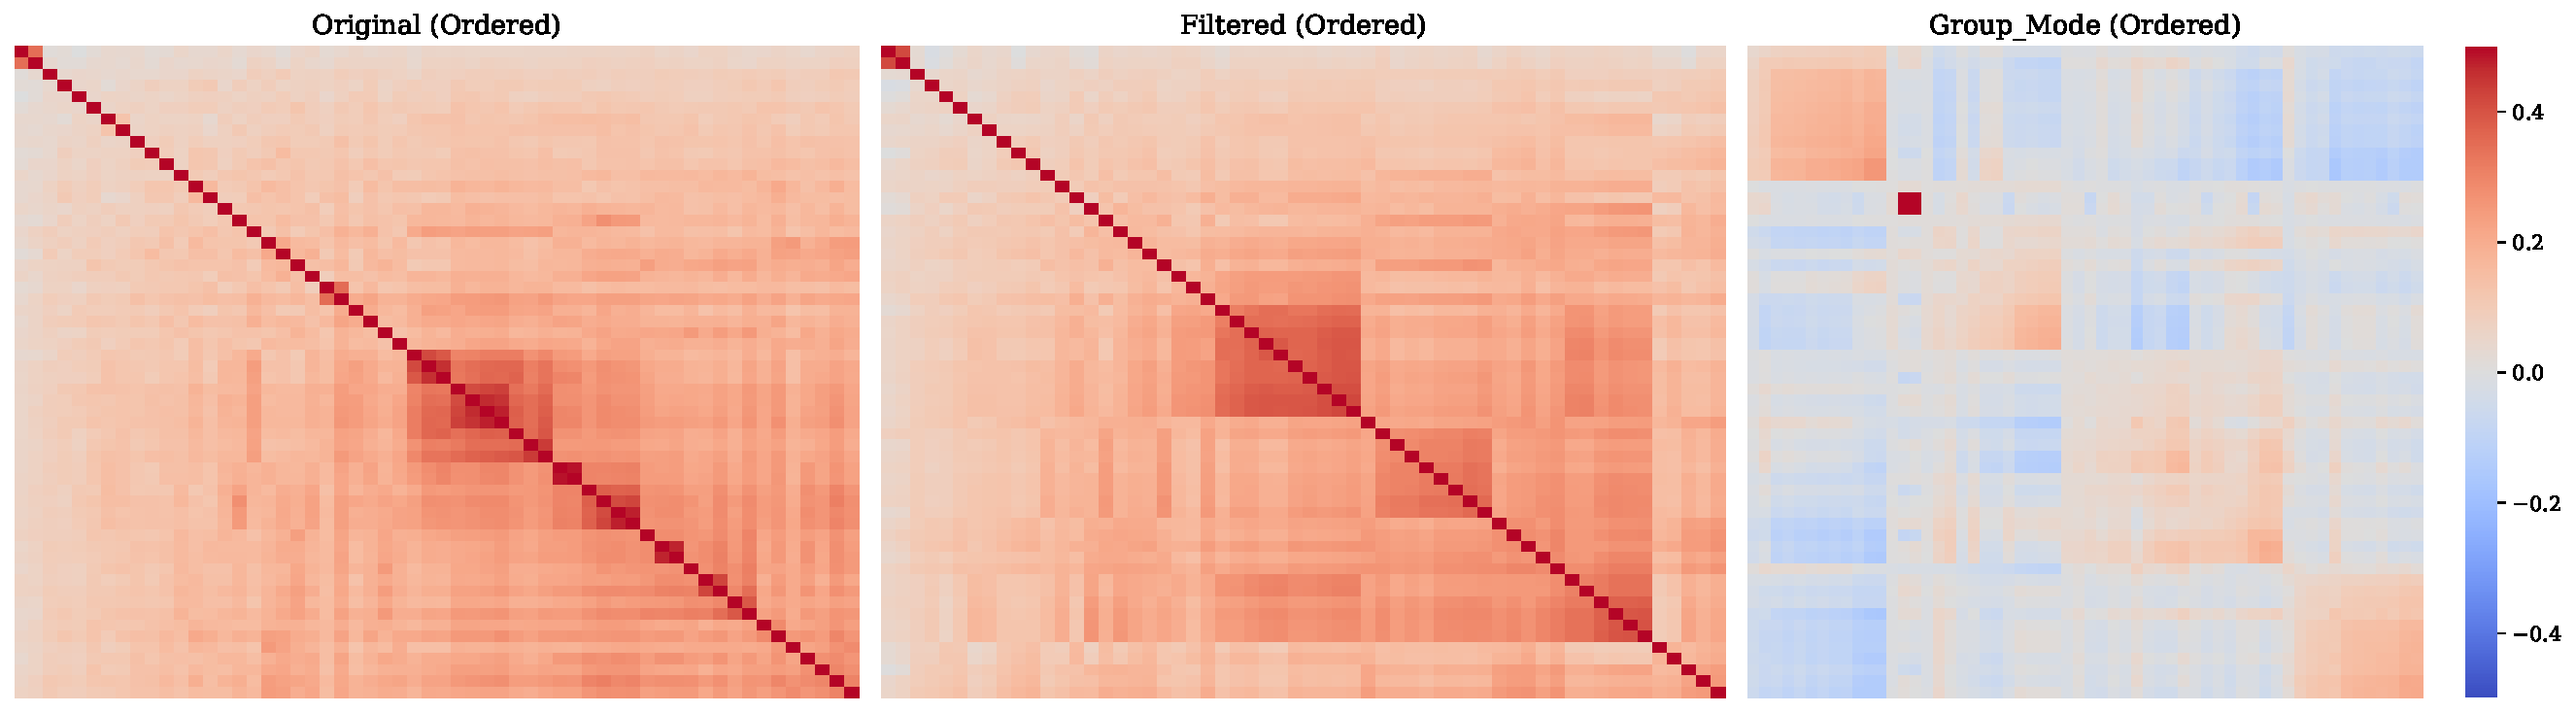
\includegraphics[
  width=\linewidth,
  height=0.72\textheight,
  keepaspectratio
]{images/figure_10_ordered_heatmaps.pdf}
\captionof{figure}{Ordered heatmaps for original and RMT-filtered correlation matrices. Panel titles are enlarged and the common color scale makes the group-mode blocks directly comparable with the original and retained structures.}
\label{fig:ordered_heatmaps}
\end{center}

\subsection{Dendrogram comparison}

Dendrograms give another view of the same distance geometry. We show the group-mode tree in Figure~\ref{fig:dendrograms}, because it is the representation that most directly addresses the structural question after market-mode removal. The colors identify the initial macro-sector classification, making the figure a visual diagnostic rather than a sector-assignment rule. Table~\ref{tab:cophenetic_summary} retains the original, filtered and group-mode fit summaries; the full three-tree comparison is supplementary material.


\begin{center}
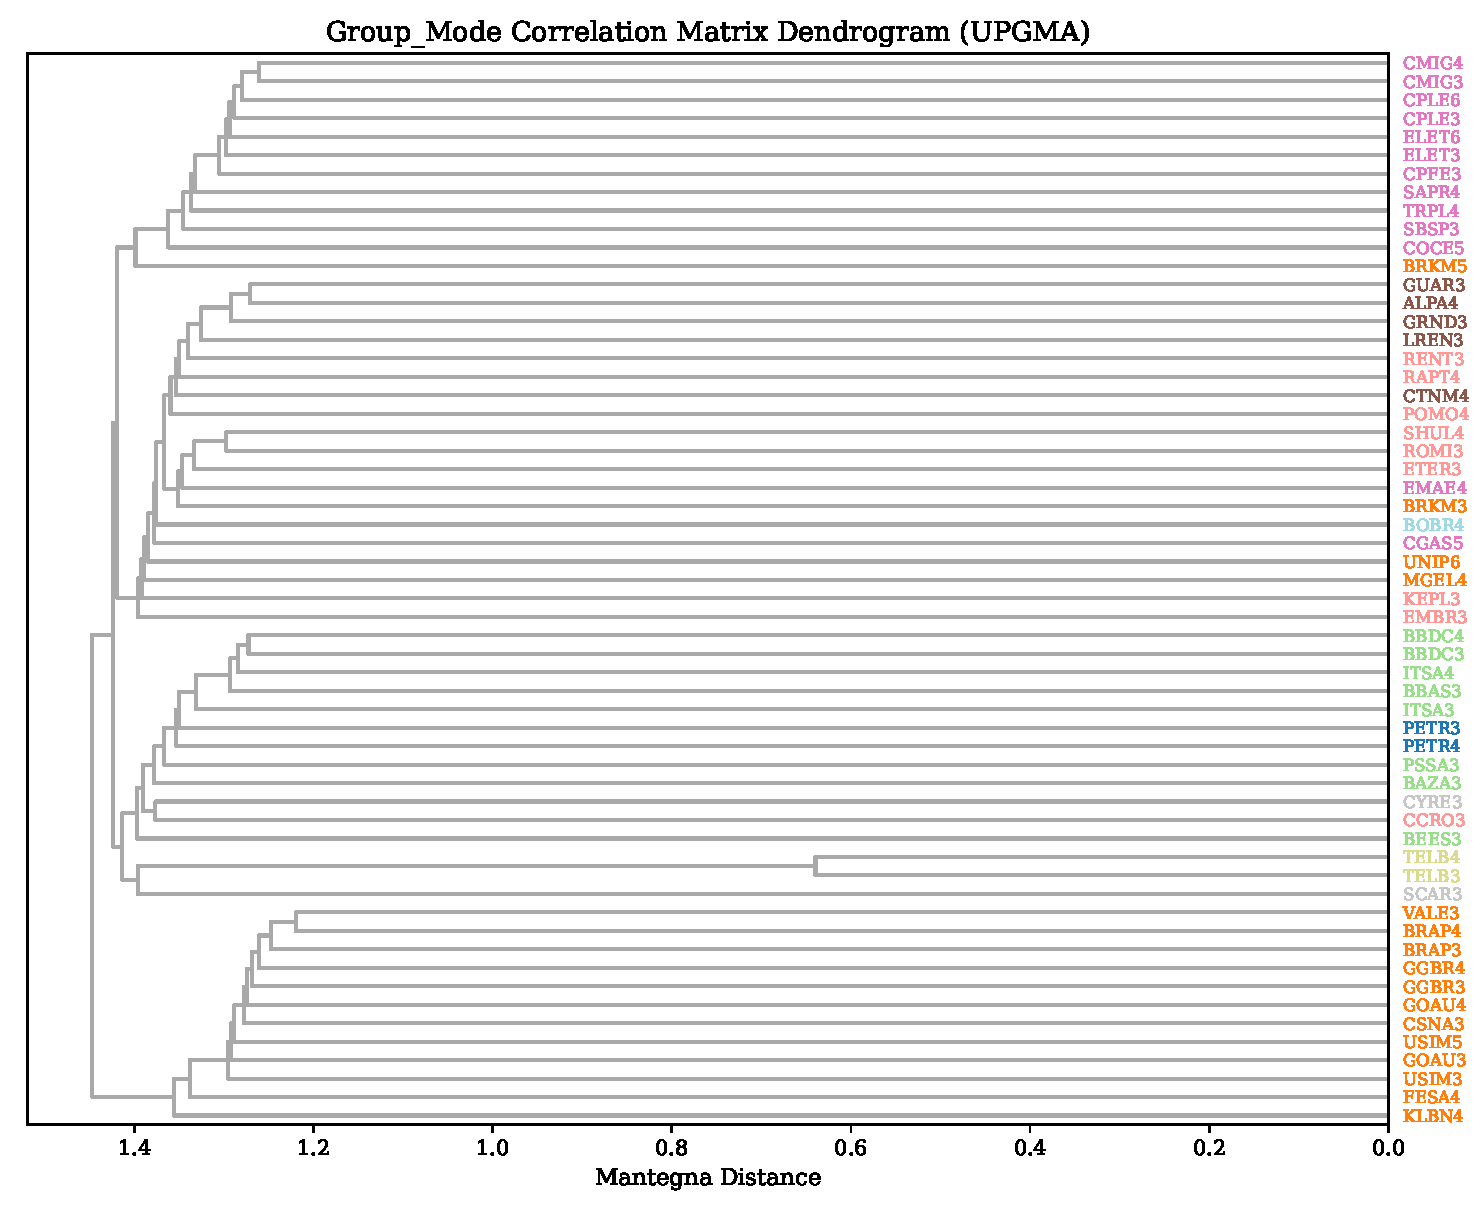
\includegraphics[
  width=\linewidth,
  height=0.8\textheight,
  keepaspectratio
]{images/figure_9_group_mode_dendrogram.pdf}
\captionof{figure}{Group-mode correlation-matrix dendrogram using Mantegna distances and average linkage. It summarizes the localized geometry remaining after the broad market component is removed; colored labels indicate the initial macro-sector classification.}
\label{fig:dendrograms}
\end{center}

\begin{center}
\captionof{table}{Cophenetic correlations for hierarchical clustering.}
\label{tab:cophenetic_summary}
\begin{tabular}{lrr}
\toprule
Matrix & Assets & Cophenetic correlation \\
\midrule
Original & 58 & 0.950 \\
Filtered & 58 & 0.934 \\
Group Mode & 58 & 0.871 \\
\bottomrule
\end{tabular}
\end{center}
\GlobalPrecisionNote

The cophenetic correlation is highest for the original matrix, 0.950, and remains high for the filtered matrix, 0.934. The group-mode value is lower, 0.871. Removing the leading market component reduces the smooth common structure that is easiest for a tree to summarize. The lower value therefore indicates a less tree-like group-mode geometry, not an absence of localized organization.

The clustering results connect naturally to network filtering. Ordered heatmaps and dendrograms suggest that localized structure remains after RMT filtering. We next examine how this structure appears when only the strongest distance-ranked edges are retained under MST and PMFG constraints.
